\documentclass{standalone}
\usepackage{tikz}
\begin{document}
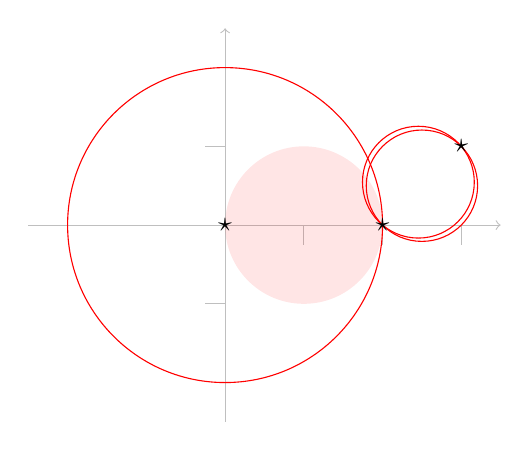
\begin{tikzpicture}
\draw [->, gray!50] (-2.5, 0) to (3.5, 0);
\draw [->, gray!50] (0, -2.5) to (0, 2.5);
\draw [gray!50] (1,0) to (1,-.25);
\draw [gray!50] (2,0) to (2,-.25);
\draw [gray!50] (3,0) to (3,-.25);
\draw [gray!50] (0,1) to (-.25, 1);
\draw [gray!50] (0,-1) to (-.25, -1);
\fill [red, very nearly transparent] (1,0) circle (1);
\draw [red] (2.45506,0.544937) circle (0.709957);
\draw [red] (2.5,0.5) circle (0.7071);
\draw [red] (0,0) circle (2);
\node at (0,0) {$\star$} ;
\node at (2,0) {$\star$} ;
\node at (3,1) {$\star$} ;
\end{tikzpicture}
\end{document}
